\begin{defnbox}\nospacing
    \begin{defn}[\hfill\pythoninline{import torch._functorch.aot_autograd}\newline A Tensor Library\hfill\tcblack{[ATen]}]
        \label{defn:aten_a_tensor_library}\leavevmode\\
        \begin{minipage}{0.56\textwidth}
            PyTorch consists of roughly 2000+ operations.
            A Tensor Library is a low level C++ interface Tensor library, that decomposes the Python API operations into fundamental operations.
            During eager mode PyTorch routes its normal function calls to ATen library calls.
       \end{minipage}\hfil
        \begin{minipage}{0.4\textwidth}
            \begin{figure}[H]
                \centering
                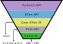
\includegraphics[width=1.0\textwidth]{pytorch_submodule/src/the_framework/graph_acquisition/figures/ATen.pdf}
            \end{figure}
        \end{minipage}
        \begin{mintlinebox}{python}
            torch.ops.aten.mse_loss.default(|\texttt{\optc{ATenTensor1}}|,|\texttt{\optc{ATenTensor2}}|)
        \end{mintlinebox}
        \begin{circlelistnosep}
            \item ATen IR: The whole ATen library
            \item Core ATen IT: is a smaller subset of ATen IR operations
            \item Prims IR: is a smaller subset of Core ATen IR operations
            \item Device IR: are the actual device primitives
        \end{circlelistnosep}
    \end{defn}
\end{defnbox}
\begin{questionbox}[Why Do We need Hierachical Operations?]\nospacing
    If we want to support PyTorch operations on a new harware accelerator it would be nearly impossible to support the full list of PyTorch API in hardware.
    But we could build a compiler that supports one of the smaller subset of fundamental operators defined in Core Aten IR or Prims IR.
\end{questionbox}


%%% Local Variables:
%%% mode: latex
%%% TeX-command-extra-options: "-shell-escape"
%%% TeX-master: "../../../../../formulary"
%%% End:
